\chapter{Choosing a City as an Entrepreneurial Constraint}

In this School of Hard Knocks segment, James gives a countdown of five cities for starting a business and becoming an entrepreneur in 2021. The useful way to read the lecture is not as a travel list, but as a sequence of location judgments. A city changes the founder's operating environment: it changes costs, customers, capital, talent, networking, policy, and the surrounding entrepreneurial culture. We will keep the countdown order, but we will make explicit the decision logic that is already present in the spoken argument.

\paragraph{Source note.}
The spoken source is a School of Hard Knocks entrepreneurship video, curated for this book by LazyingArt LLC through Video2Book. No validated board, chart, or diagram screenshots were retained for this lecture, so the visual material below is reconstructed from the transcript rather than copied from the video.

\section{The Ranking Problem}

James begins by saying that the ranking is based on an accumulation of factors. Before he names a city, he names the variables: opportunities, startup cost, cost of living, growth and profit potential, networking, and client opportunities. That opening gives the lecture its spine. We are not asking for the cheapest city, or the largest city, or the most famous startup city. We are asking how a founder should compare whole ecosystems.

Let \(c\) denote a candidate city. A cautious mathematical shorthand for the spoken reasoning is
\begin{equation}
S(c)
=
w_oO(c)
+w_sS_c(c)
+w_lL(c)
+w_gG(c)
+w_nN(c)
+w_mM(c)
+w_kK(c)
+w_pP(c).
\end{equation}
Here \(S(c)\) is a reconstructed qualitative city score. The terms stand for opportunity \(O\), startup-cost conditions \(S_c\), cost-of-living conditions \(L\), growth and profit potential \(G\), networking access \(N\), market or client access \(M\), capital access \(K\), and policy or tax conditions \(P\). This is not a formula James computes in the video. It is a bookkeeping device for the tradeoffs he narrates.

The countdown itself is the first piece of data:
\begin{equation}
\text{Seattle}=5,\qquad
\text{Denver}=4,\qquad
\text{Los Angeles}=3,\qquad
\text{Miami}=2,\qquad
\text{Austin}=1.
\end{equation}
The order is not incidental. The lecture moves from strong but costly ecosystems toward places where James sees more advantages aligning at once.

\begin{figure}
\centering
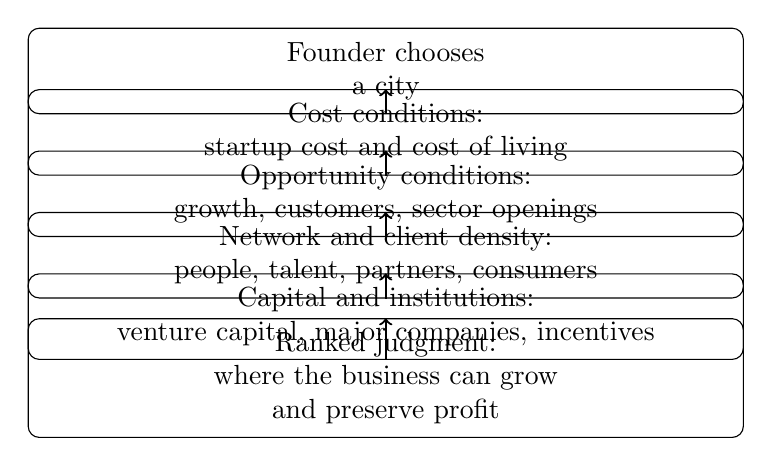
\begin{tikzpicture}[
  node distance=0.78cm,
  every node/.style={draw, rounded corners, align=center, text width=0.72\linewidth, inner sep=5pt},
  arrow/.style={->, thick}
]
\node (a) {Founder chooses\\a city};
\node (b) [below of=a] {Cost conditions:\\startup cost and cost of living};
\node (c) [below of=b] {Opportunity conditions:\\growth, customers, sector openings};
\node (d) [below of=c] {Network and client density:\\people, talent, partners, consumers};
\node (e) [below of=d] {Capital and institutions:\\venture capital, major companies, incentives};
\node (f) [below of=e] {Ranked judgment:\\where the business can grow\\and preserve profit};
\draw[arrow] (a) -- (b);
\draw[arrow] (b) -- (c);
\draw[arrow] (c) -- (d);
\draw[arrow] (d) -- (e);
\draw[arrow] (e) -- (f);
\end{tikzpicture}
\caption{A transcript-derived reconstruction of the location-choice logic. The lecture does not show this as a board diagram, but the spoken ranking follows this cumulative structure.}
\end{figure}

\section{Seattle: Growth, Tech Gravity, and Cost}

The countdown starts at number five with Seattle. James describes Seattle as one of the fastest-growing cities in the United States and as a city already known for technology. The new point in the lecture is that Seattle is also becoming a fast-growing startup hub.

Then the first serious tradeoff appears. Seattle has a high cost of living. James does not hide that fact. His claim is that the city's economic development and growing venture capital scene can offset some of the burden. In our notation, the Seattle case has the form
\begin{equation}
K(\text{Seattle})+G(\text{Seattle})+N(\text{Seattle})
\quad \hbox{partly offset} \quad
L(\text{Seattle}).
\end{equation}
The word ``partly'' matters. The lecture is not saying that cost disappears. It is saying that capital access, growth, technology, and a young entrepreneurial crowd may make the cost tolerable for some founders.

\section{Denver: Incentives and Sector Investment}

At number four, James moves to Denver, Colorado. The reasoning broadens. Denver is described as a top-ten city for starting a business and also as a top-ten city for startups. The transcript then points to government tax incentives and multi-billion-dollar investment across industries such as manufacturing, transportation, cannabis, and related sectors.

This portion of the transcript repeats and breaks in places, so the clean note should preserve the intended claim without multiplying it. Denver's role in the ranking is to show that a founder's ecosystem is not only about venture capital or famous technology companies. Public incentives, industry-specific investment, livability, and the attraction of young workers can also enter the calculation.

A compact way to write Denver's contribution is
\begin{equation}
S(\text{Denver})
\quad \hbox{rises with} \quad
P(\text{Denver})+O(\text{Denver})+G(\text{Denver}),
\end{equation}
where \(P\) captures the policy and incentive environment, \(O\) captures opportunity, and \(G\) captures the growth potential implied by sector investment.

\section{Los Angeles: Network Value Against High Cost}

At number three, James names Los Angeles. Here the lecture sharpens its central tension. Los Angeles is described as one of the largest cities for tech entrepreneurship and as the third largest city for startups in the United States. It has consumers, like-minded people, access to a broad market, and concentrated talent. But it is also expensive.

This is the place in the lecture where the ranking stops looking like a simple cost comparison. If low cost were the only variable, Los Angeles would be hard to justify. James's point is that network and market access change the calculation. They do not make the cost vanish, but they can raise the possible upside of being there.

\subsection{Question \& Answer}

\paragraph{Question.}
Why can an expensive city still rank highly for an entrepreneur?

\paragraph{Answer.}
Because cost is only one term in the founder's environment. A high-cost city may still be worth considering when its network, market, talent, and customer access improve the chance that the business can grow. The Los Angeles argument can be summarized as
\begin{equation}
N(c)+M(c)+G(c)+K(c)
\quad \hbox{can outweigh} \quad
L(c),
\end{equation}
provided those positive terms are strong enough.

For Los Angeles specifically, James's argument is that the city offers a large consumer base, a wide market, and a dense pool of talent and like-minded people. The cost penalty remains real, and that is why Los Angeles stays at number three rather than rising higher in his ranking. But the conceptual lesson is durable: a founder is not buying cheapness; a founder is buying access.

\section{Miami: Density, Collaboration, and Institutions}

The pivot from Los Angeles to Miami moves the lecture from network value to ecosystem density. James calls Miami an incredible place to start a business and says it has the highest density of startups in the country. He also emphasizes creativity, collaboration, and the ability of businesses to innovate, develop, and grow there.

The concrete institutional claim is
\begin{equation}
\#\{\hbox{Inc. 5000 companies in Miami}\}=139.
\end{equation}
He also points to venture capital support and says Miami ranks as a top-five fastest-growing city in the United States. The Miami case is cumulative rather than single-cause. Its score is not one large term; it is a cluster of reinforcing terms:
\begin{equation}
S(\text{Miami})
\approx
\hbox{startup density}
+\hbox{collaboration}
+\hbox{institutions}
+\hbox{capital}
+\hbox{city growth}.
\end{equation}
This approximation is not a measured formula. It is a disciplined shorthand for James's sequence of claims: density brings people together, collaboration helps businesses develop, institutions supply credibility and support, and capital helps firms grow.

\section{Austin: The Combined Case for Number One}

The final city is Austin, Texas. James presents Austin as the number-one city on his list, and the argument works because it gathers many earlier variables into one place. He describes Austin as the fastest-growing city in the United States, says CNBC ranked it as the number-one city to start a business in 2021, and states that Austin has grown its startups faster than any city in the country by 81 percent.

The spoken growth claim is
\begin{equation}
\hbox{Austin startup growth}=81\%.
\end{equation}
James then adds affordability, opportunity, networking, consumer availability, startup culture, and tax conditions. As stated in the lecture,
\begin{equation}
\hbox{state income tax}=0,
\qquad
\hbox{corporate tax rate}=0\%.
\end{equation}
These are speaker-attributed claims from the transcript, not tax advice. Their function in the lecture is to make policy part of the founder's profit environment.

\paragraph{Worked example: score updates.}
A useful way to track the lecture's reasoning is to imagine a score being updated as evidence is added. We begin with a neutral assessment \(S_0(c)\). Then each class of evidence changes the score:
\begin{align}
S_1(c) &= S_0(c)+\Delta_{\text{growth}}(c),\\
S_2(c) &= S_1(c)+\Delta_{\text{network}}(c)+\Delta_{\text{clients}}(c),\\
S_3(c) &= S_2(c)+\Delta_{\text{capital}}(c)+\Delta_{\text{institutions}}(c),\\
S_4(c) &= S_3(c)+\Delta_{\text{policy}}(c)-\Delta_{\text{cost}}(c).
\end{align}
For Austin, James's conclusion is that the positive increments dominate. Growth, startup culture, affordability, tax conditions, consumer access, network opportunity, and a supportive local business culture all point in the same direction. That is why Austin functions as the payoff of the countdown rather than merely another entry in the list.

\section{The Ranking in One View}

The lecture is not a spreadsheet, but the spoken evidence is compact enough to arrange in a narrow table. The point of the table is not to replace the narrative. It is to keep the claims visible while preserving the countdown order.

\begin{table}
\centering
\begin{tabular}{p{0.10\linewidth}|p{0.16\linewidth}|p{0.34\linewidth}|p{0.30\linewidth}}
Rank & City & Main stated advantages & Constraint or concrete claim \\
\hline
5 & Seattle &
Tech hub; fast-growing startup hub; venture capital scene; young, innovative crowd &
High cost of living, partly offset in the speaker's view by development and capital access \\
\hline
4 & Denver &
Top-ten business and startup city; tax incentives; sector investment in manufacturing, transportation, cannabis, and more &
Transcript repeats here; preserve the policy and sector-opportunity claim once \\
\hline
3 & Los Angeles &
Large tech entrepreneurship city; third largest startup city; consumers, talent, global market access, and network density &
Very high cost of living keeps it at number three \\
\hline
2 & Miami &
Startup-density claim; creative and collaborative culture; institutional support; venture capital support &
Speaker states 139 Inc. 5000 companies and top-five fastest-growing-city status \\
\hline
1 & Austin &
Fastest-growing-city claim; CNBC number-one claim; startup culture; affordability; networking; supportive business culture &
Speaker states 81 percent startup growth, no state income tax, and zero percent corporate tax rate \\
\end{tabular}
\caption{Transcript-backed ranking evidence, arranged as a compact founder-location screen.}
\end{table}

\section{Summary}

The lecture's practical lesson is that location is part of entrepreneurship strategy. We are not merely asking where rent is lowest or where the skyline is most famous. We are asking where opportunity, cost, network, customers, capital, institutions, taxes, and culture combine in a way that lets a business start and grow.

The countdown develops that lesson step by step. Seattle introduces tech gravity and venture capital against high cost. Denver adds incentives and sector investment. Los Angeles forces the central question: when can network and market access justify expense? Miami adds density, collaboration, institutions, and venture capital support. Austin closes the argument by combining growth, affordability, policy advantages, consumer access, networking, and supportive entrepreneurial culture into the speaker's number-one choice.